% ============================================================
% main.tex — "Stale Queues, Noisy Sizes"
%
% LOCAL COMPILATION
%   latexmk -pdf main.tex
%   (requires: texlive-latex-recommended texlive-latex-extra
%              texlive-fonts-recommended texlive-bibtex-extra)
%   Or manually:
%     pdflatex main.tex && bibtex main && pdflatex main.tex && pdflatex main.tex
%
% OVERLEAF
%   Upload the contents of this paper/ directory.
%   Set the main document to main.tex.
% ============================================================

\documentclass[11pt]{article}

\usepackage[margin=1in]{geometry}
\usepackage{float}
\usepackage{booktabs}
\usepackage{graphicx}
\usepackage{amsmath}
\usepackage{amssymb}
\usepackage{microtype}
\usepackage{xcolor}
\usepackage{caption}
\usepackage{subcaption}
\usepackage{natbib}
\usepackage[colorlinks=true, linkcolor=blue!60!black,
            citecolor=blue!60!black, urlcolor=blue!60!black]{hyperref}
\usepackage{listings}
\usepackage{array}

\graphicspath{{./figures/}{../exp2/figures/}}

% ---- listings style for inline code ----
\lstset{
  basicstyle=\ttfamily\small,
  columns=flexible,
  keepspaces=true,
}

% ---- caption style ----
\captionsetup{font=small, labelfont=bf}

% ---- title ----
\title{\textbf{Stale Queues, Noisy Sizes:\\
       Can LLMs Discover Better Dispatch Strategies?}}

\author{Kai Xu\\[2pt]
        \small New York University}

\date{}

% ============================================================
\begin{document}
\maketitle

% ============================================================
\begin{abstract}
Real-world load-balancing problems often diverge from textbook setups:
queue-length reports may be stale, job-size estimates may be
unreliable, or a standard algorithm may degrade under a
problem-specific failure mode that requires a novel correction.
When practitioners encounter such scenarios, they increasingly turn to
large language models for help. However, it is unclear whether LLMs can
reason correctly about the stochastic properties that make these
problems hard.
We investigate this through two controlled experiments in which six
LLMs zero-shot write dispatch functions for a server farm under
heartbeat staleness and under noisy SRPT routing respectively.
Across both experiments: no model reliably beats the best classical
baseline in median performance, and naive deployment of LLM-generated
functions frequently performs \emph{worse} than the algorithm being
replaced; scale determines code validity below roughly 8B parameters
but does not predict median quality above that threshold; larger
models occasionally discover high-quality solutions that smaller
models never reach, even when their typical output is no better;
and providing an explicit description of the failure mode increases
the rate of correct solutions but still does not produce reliable
improvements.
These findings suggest that LLMs carry useful latent knowledge about
algorithmic design but cannot yet be trusted to improve a deployed
load-balancing algorithm without human oversight.
\end{abstract}

% ============================================================
\section{Introduction}
\label{sec:intro}

A dispatcher routing jobs to a server farm always operates on imperfect
information.
Two failure modes motivate this paper.
First, queue-length reports may be stale: by the time a heartbeat
arrives from a worker, that worker has already processed additional
jobs, and routing greedily on the stale report overloads whichever
worker happened to report a short queue.
Second, even with fresh state, the dispatcher may not know how long
an incoming job will take and must rely on a noisy size estimate;
the standard SRPT heuristic degrades when estimates are severely
wrong.

Both scenarios reflect a common practical situation: an engineer
knows that a standard algorithm applies but suspects it is
underperforming, and turns to an LLM for a better alternative.
Recent work shows LLMs can discover non-obvious algorithmic
strategies when suitably prompted
\citep{fawzi2024funsearch, novikov2025alphaevolve, ma2024eureka},
but these successes typically involve iterative search or explicit
feedback.
We ask whether zero-shot prompting alone is sufficient, and whether
the answer changes when the LLM is told what is breaking.
We test this with six models across two experiments: Experiment~1
on age-aware dispatch under heartbeat staleness, and Experiment~2
on adapting SRPT routing when job-size estimates are heavily noisy.

Our main findings are:
\begin{enumerate}
  \item \textbf{No model reliably beats the best classical baseline.}
    In Experiment~1, every model's median performance is worse than
    routing uniformly at random (the weakest possible baseline).
    In Experiment~2, median performance sits between Least Connections
    and SRPT-noisy; only a small minority of trials improve on
    SRPT-noisy.
    Naively deploying LLM-generated functions can produce results
    substantially worse than the algorithm being replaced.
  \item \textbf{Scale gates code validity but not median quality.}
    Below roughly 8B parameters, models rarely produce valid,
    executable dispatch functions.
    Above that threshold, larger models do not achieve better median
    performance: the largest Qwen3 model (14B) does not outperform
    smaller models in either experiment.
  \item \textbf{Scale does affect the extremes.}
    Larger models occasionally discover high-quality solutions that
    smaller models never find, even when their typical output is no
    better.
    The correct strategy in each experiment appears in only a small
    fraction of trials, concentrated in the larger models.
  \item \textbf{Describing the failure mode helps, but is not sufficient.}
    Experiment~2's prompt explicitly names the phantom-underload
    failure; the rate of correct solutions is much higher than in
    Experiment~1, but median performance still does not reliably
    exceed the best baseline.
\end{enumerate}

% ============================================================
\section{Related Work}
\label{sec:related}

\paragraph{Load balancing under staleness.}
Join-Shortest-Queue (JSQ)~\citep{ahn1996jsq} is optimal under
complete, instantaneous state information.
Under stale reports, JSQ is susceptible to the thundering herd:
all dispatchers simultaneously route to whoever last reported a short
queue, overloading that worker until the next heartbeat resets the
picture.
Power-of-Two-Choices~\citep{mitzenmacher2001power} disrupts herding
by sampling two workers and routing to the shorter, trading
information for robustness.
\citet{mitzenmacher2000useful} shows that even moderately outdated
information can eliminate Po2C's guarantees.
\citet{dahlin2000stale} characterizes the herding failure analytically
and derives age-adjusted routing thresholds, the same kind of
correction our experiments ask LLMs to discover independently.

\paragraph{SRPT scheduling and estimation noise.}
\citet{schrage1968srpt} proved that preemptive SRPT minimizes mean
response time in the M/G/1 queue; this optimality requires exact
job sizes.
In practice, job sizes must be estimated, and estimation errors
degrade performance.
Heavy-tailed service times, common in real workloads
\citep{crovella1997selfsimilar}, amplify the damage because large
jobs are common enough to be persistently present, and a severe
underestimate on a large job creates a long-lasting phantom underload.

\paragraph{LLMs for algorithm synthesis.}
\citet{fawzi2024funsearch} and \citet{novikov2025alphaevolve} use
LLM-driven search to discover improvements to combinatorial
optimization and data-center scheduling, achieving substantial gains
over human-designed baselines.
\citet{ma2024eureka} synthesizes reward functions for reinforcement
learning zero-shot from problem descriptions alone.
\citet{cheng2025letbarbarians} examine LLM-generated heuristics for
scheduling problems in a systems context.
Our work differs in two respects: correctness is determined by
steady-state simulation rather than test cases or human evaluation,
and we study zero-shot synthesis without iterative search or feedback,
which represents the more common case when a practitioner queries
an LLM for algorithm advice.

\paragraph{AI for systems.}
Sparrow~\citep{ousterhout2013sparrow} implements Po2C in a real
cluster scheduler, showing the two-choices principle works at
production scale.
\citet{cheng2025barbarians} surveys AI-driven systems research and
reports 5$\times$ speedups on load-balancing tasks via LLM-guided
search.
Our setting is simpler than production cluster scheduling, which lets
us isolate the reasoning challenge cleanly: one dispatch decision per
job, one integer output, full-simulation evaluation.

% ============================================================
\section{Experiment 1: Age-Aware Dispatching under Heartbeat Staleness}
\label{sec:exp1}

\subsection{System Model}
\label{sec:exp1-setup}

We simulate a single dispatcher routing to $N{=}8$ workers.
Jobs arrive as a Poisson process at total rate $\lambda{=}6.4$\,jobs/ms
($\rho{=}0.8$).
Service times are i.i.d.\ Exponential(mean 1\,ms).
Each worker maintains an independent FIFO queue.

Each worker emits a heartbeat every $H{=}20$\,ms.
Each heartbeat incurs a propagation delay drawn from
$\mathrm{Uniform}(1,5)$\,ms.
The dispatcher records the reported queue length and the arrival time
of the most recent heartbeat.
At dispatch time $t$, worker $w$'s heartbeat age is
$a_w = t - \text{last\_heard}_w$, ranging from near zero to nearly
$H{+}5$\,ms.
Mean age at dispatch is approximately 11--12\,ms, or roughly 11--12
expected completions of staleness.

\paragraph{Dispatcher interface.}
\begin{lstlisting}
def dispatch(queue_lengths: list[int],
             queue_ages_ms: list[float],
             num_workers:   int) -> int
\end{lstlisting}
\texttt{queue\_lengths[w]} is the stale reported queue depth;
\texttt{queue\_ages\_ms[w]} is the age in milliseconds of the most
recent report.
The function returns the worker index to receive the incoming job.

\paragraph{Metric.}
We sample the true queue depths every 10\,ms and compute the
cross-worker standard deviation $\sigma$.
We report mean $\sigma$ over $10^5$ jobs; lower is better.
Each strategy is evaluated over 100 independent seeds.

\subsection{Baselines}
\label{sec:exp1-baselines}

Three classical policies serve as reference points:
\begin{itemize}
  \item \textbf{Random.} Route uniformly at random.
    Any strategy worse than Random is actively harmed by the
    information it uses.
  \item \textbf{Po2C (stale).} Sample two workers and route to the
    shorter reported queue~\citep{mitzenmacher2001power}.
    Disrupts herding at the cost of ignoring ages entirely.
  \item \textbf{JSQ (stale).} Route to the minimum reported queue,
    breaking ties randomly.
    Uses stale queue lengths greedily; highly susceptible to
    the thundering herd.
\end{itemize}

JSQ (stale) achieves median $\sigma{=}14.95$, nearly four times worse
than Random ($\sigma{=}3.77$).
Figure~\ref{fig:herd} shows the mechanism directly: one or two workers
repeatedly spike above 50 jobs while others idle, resetting each
heartbeat cycle.
Po2C reduces imbalance to $\sigma{=}4.40$ through randomization but
leaves age information entirely unused.

\begin{figure}[H]
  \centering
  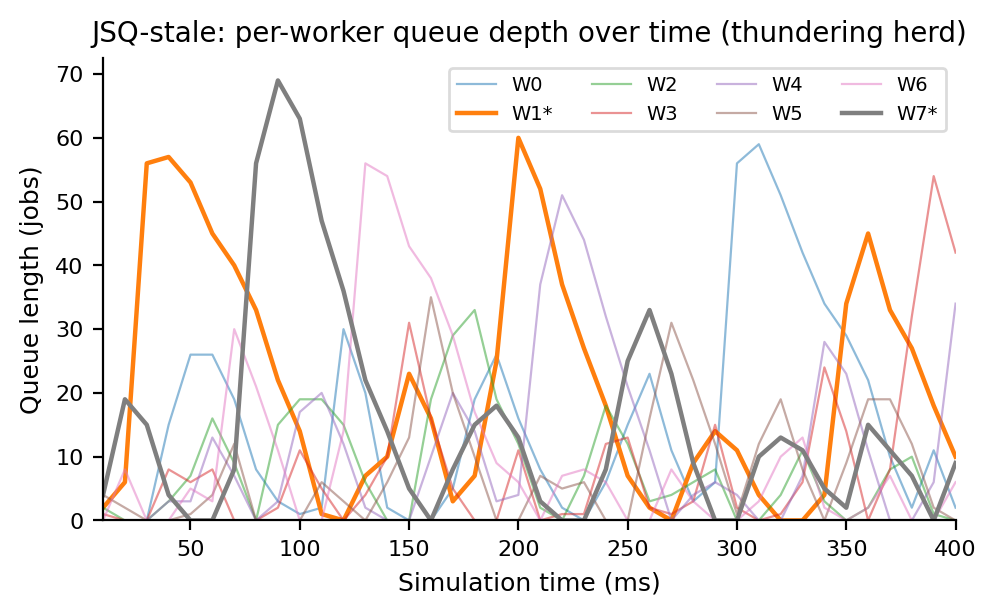
\includegraphics[width=\linewidth]{fig1_thundering_herd}
  \caption{%
    \textbf{Thundering herd under JSQ-stale.}
    Per-worker true queue depth over 400\,ms (seed~0).
    One or two workers repeatedly spike above 50 jobs while the rest
    idle.
    Each spike resets when a heartbeat reassigns the apparent
    shortest-queue label.
    JSQ-stale ($\sigma{=}14.95$) performs nearly four times worse than
    Random ($\sigma{=}3.77$).
  }
  \label{fig:herd}
\end{figure}

\subsection{LLM Evaluation}
\label{sec:exp1-llms}

We evaluate six models: Qwen3-1.7B, Qwen3-4B, Qwen3-8B, Qwen3-14B,
DeepSeek-R1-0528-Qwen3-8B (hereafter DeepSeek-R1), and gpt-oss-20b.
Each model is prompted at temperature 1 to write the body of the
\texttt{dispatch} function, given the system parameters and interface
docstring.
No strategy is suggested, no examples are provided, and the thundering
herd is not named.
Responses are parsed by extracting content between \texttt{<code>}
tags.

Each generated function is paired with a fixed simulation seed and
evaluated for 100 independent trials per model.
A trial is valid if the code parses, executes without error on every
dispatch call, and returns an integer in $[0, N)$.
Parse rates range from 20\% to 84\%, yielding 257 valid trials in total
(Table~\ref{tab:exp1-results}).

\subsection{Results}
\label{sec:exp1-results}

\paragraph{No model reliably beats Random.}
Table~\ref{tab:exp1-results} shows median mean~$\sigma$ across valid
trials.
Every model performs substantially worse than Random.
The best median is 21.0 (gpt-oss-20b), $5.6\times$ worse than Random
and $4.8\times$ worse than Po2C.
There is no clear scaling relationship: Qwen3-8B (24.0) outperforms
the larger Qwen3-14B (27.4), and gpt-oss-20b achieves the best median
despite the lowest parse rate.
Figure~\ref{fig:dist} shows the per-trial distribution for each model.

\begin{table}[H]
\centering
\caption{%
  Experiment~1 results.
  Median mean~$\sigma$ over 100 seeds for baselines and over all
  valid trials for LLMs. Lower is better.
  $^\dagger$Reported parameter count from model metadata.
}
\label{tab:exp1-results}
\smallskip
\begin{tabular}{lrrrc}
\toprule
\textbf{Strategy / Model} & \textbf{Params} & \textbf{Parse\%} &
  \textbf{$n$} & \textbf{Med.\ $\sigma$} \\
\midrule
\multicolumn{5}{l}{\textit{Classical baselines (100 seeds)}} \\
\quad Random       & ---   & --- & 100 & 3.77 \\
\quad Po2C (stale) & ---   & --- & 100 & 4.40 \\
\quad JSQ (stale)  & ---   & --- & 100 & 14.95 \\
\midrule
\multicolumn{5}{l}{\textit{LLM-generated dispatchers}} \\
\quad Qwen3-1.7B       & 1.8B  & 84\% &  82 & 27.21 \\
\quad Qwen3-4B         & 4.0B  & 55\% &  40 & 26.75 \\
\quad Qwen3-8B         & 8.5B  & 43\% &  36 & 24.02 \\
\quad Qwen3-14B        & 15.7B & 68\% &  60 & 27.38 \\
\quad DeepSeek-R1 (8B) & 8.5B  & 45\% &  29 & 27.26 \\
\quad gpt-oss-20b      & 20B$^\dagger$ & 20\% & 10 & 21.03 \\
\bottomrule
\end{tabular}
\end{table}

\begin{figure}[H]
  \centering
  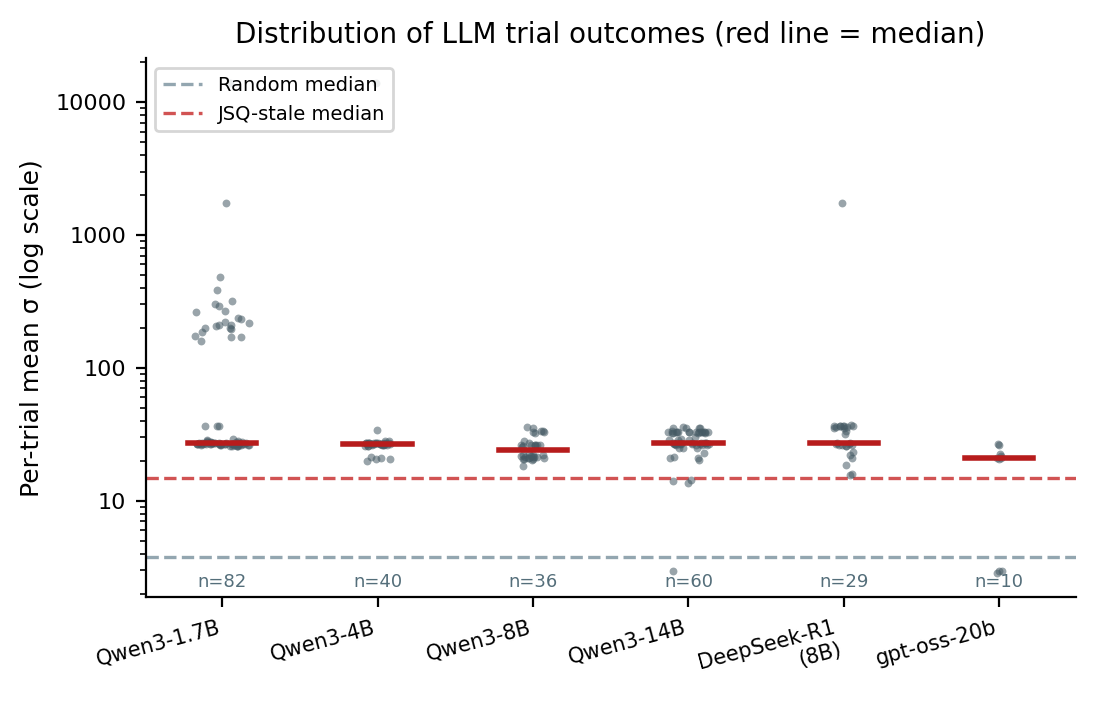
\includegraphics[width=\linewidth]{fig4_heavy_tailed_distributions}
  \caption{%
    \textbf{Per-trial $\sigma$ distributions in Experiment~1.}
    Each dot is one valid trial; the red bar marks the within-model
    median.
    Most models cluster in the $\sigma{\approx}20$--$35$ range.
    gpt-oss-20b shows a bimodal distribution: a small cluster of
    trials near the Random reference line alongside the majority
    well above it, corresponding to the rare trials that implement
    age subtraction correctly.
  }
  \label{fig:dist}
\end{figure}

\paragraph{The age-aware subtraction strategy was independently discovered.}
Four trials (three from gpt-oss-20b, one from Qwen3-14B) achieve
$\sigma{<}3.77$, beating Random.
All four implement the same strategy:
\begin{equation}
  \mathrm{adj}_w = \max\!\bigl(q_w - a_w,\; 0\bigr),
  \qquad
  \text{route to } \arg\min_w\, \mathrm{adj}_w
  \label{eq:subtract}
\end{equation}
Since the expected number of completions at worker $w$ in $a_w$\,ms is
$a_w / \mu = a_w$ (with $\mu{=}1$), subtracting $a_w$ from the stale
queue length estimates the current queue depth.
Clamping at zero handles negative estimates.
These four trials achieve $\sigma{\approx}2.9$, below Random.
Figure~\ref{fig:code} shows one representative from each model.

\begin{figure}[H]
  \centering
  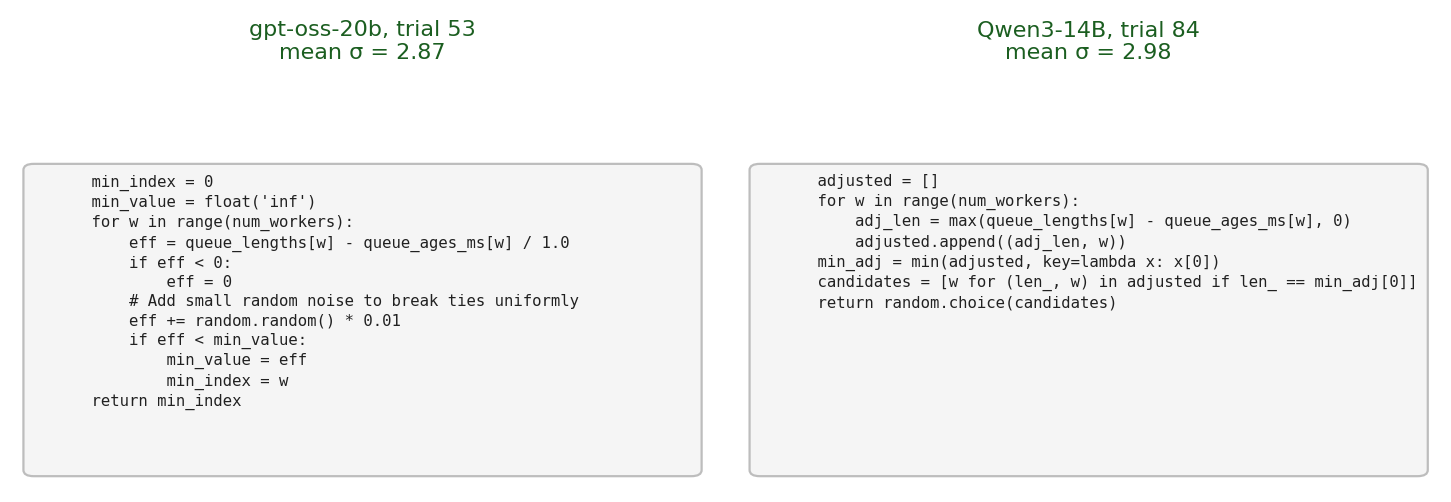
\includegraphics[width=\linewidth]{fig6_correct_strategy}
  \caption{%
    \textbf{Independent convergence on the age-subtraction strategy.}
    Two models from different families produce the same dispatch logic
    without coordination: compute $\mathrm{adj}_w = \max(q_w - a_w, 0)$,
    return $\arg\min_w\,\mathrm{adj}_w$.
    Both achieve $\sigma{\approx}2.9$, below Random's 3.77.
  }
  \label{fig:code}
\end{figure}

\paragraph{Strategy classification.}
We classify each valid trial by inspecting the generated code
(Figure~\ref{fig:strategy}):
\begin{itemize}
  \item \textbf{Subtract age} ($n{=}12$, median $\sigma{=}20.9$):
    implements $q_w - f(a_w)$ for some positive $f$.
    All four trials that beat Random belong to this class.
  \item \textbf{JSQ + age tiebreaker} ($n{=}96$, median $\sigma{=}26.7$):
    routes by shortest queue; age breaks ties only.
    Effectively reduces to JSQ-stale in practice.
  \item \textbf{Add age} ($n{=}49$, median $\sigma{=}22.1$):
    computes $q_w + \alpha \cdot a_w$.
    Interprets a long silence as evidence of load rather than as
    staleness, reversing the correct direction.
  \item \textbf{Other} ($n{=}100$, median $\sigma{=}32.7$):
    miscellaneous heuristics with no consistent pattern.
\end{itemize}

All four classes perform worse than Random.
The key observation is not which direction models get the sign
wrong, but that \emph{any} use of the age signal, in either direction,
consistently fails to beat the baseline that ignores it entirely.
Using stale information badly is worse than not using it at all.

\begin{figure}[H]
  \centering
  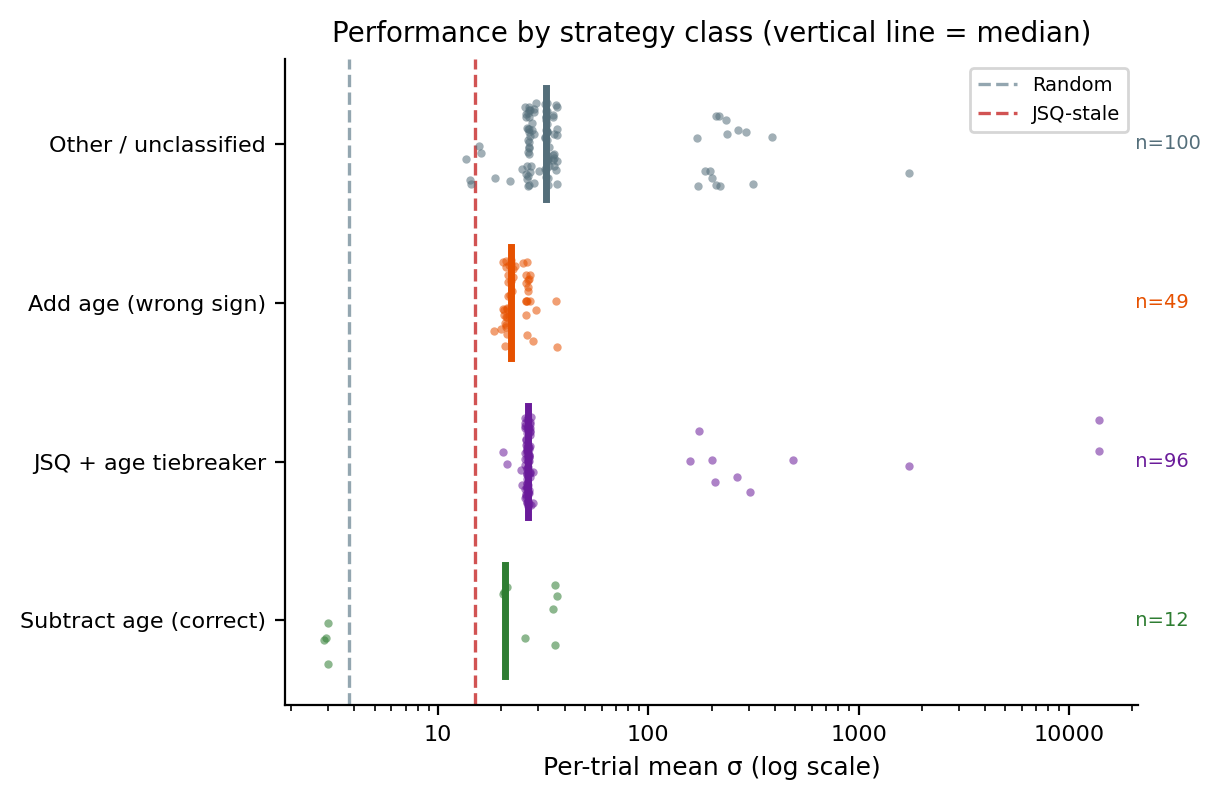
\includegraphics[width=0.9\linewidth]{fig7_strategy_class_performance}
  \caption{%
    \textbf{Performance by strategy class in Experiment~1.}
    Each dot is one valid trial; vertical bars show the within-class
    median.
    The subtract-age class contains the four trials that beat Random.
    Dashed lines mark the Random and JSQ-stale medians.
  }
  \label{fig:strategy}
\end{figure}

% ============================================================
\section{Experiment 2: Noisy SRPT Dispatching with Heavy-Tailed Jobs}
\label{sec:exp2}

\subsection{System Model}
\label{sec:exp2-setup}

The second experiment replaces heartbeat staleness with a different
source of uncertainty: noisy job-size estimates.
A single dispatcher routes jobs to $N{=}8$ workers at utilization
$\rho{=}0.8$ ($\lambda{=}6.4$\,jobs/ms).
Service times follow a Pareto distribution with shape $\alpha{=}1.5$
and mean 1\,ms.
The Pareto distribution is heavy-tailed: the probability of a job
exceeding $x$ times the mean decays as $x^{-\alpha}$, so large jobs
are substantially more common than under exponential service and
concentrate a disproportionate share of total work.

Each incoming job comes with a noisy size estimate
$\hat{S} = S \cdot \epsilon$, where $S$ is the true size and
$\epsilon = \exp(Z)$, $Z \sim \mathcal{N}(0, \sigma^2)$, $\sigma{=}1.0$.
This multiplicative noise has geometric standard deviation
$e^{\sigma} \approx 2.7$: estimates within one log-scale standard
deviation range from roughly $e^{-1} \approx 0.37\times$ to
$e^{+1} \approx 2.7\times$ the true size.

The dispatcher maintains, per worker, an accumulated estimated
remaining work (ERW):
\begin{equation}
  \mathrm{ERW}_w(t) = \sum_{j \in Q_w(t)} \hat{S}_j
  \label{eq:erw}
\end{equation}
where $Q_w(t)$ is the set of jobs currently at worker $w$.
This sum is updated when jobs arrive and depart but does not decrease
during service; the estimate is frozen at arrival.

\paragraph{Dispatcher interface.}
\begin{lstlisting}
def dispatch(connections: list[int],
             estimated_remaining_work: list[float],
             job_size_estimate: float,
             num_workers: int) -> int
\end{lstlisting}
\texttt{connections[w]} is the exact active job count at worker $w$
(no noise, no delay).
\texttt{estimated\_remaining\_work[w]} is $\mathrm{ERW}_w$, a noisy
accumulated estimate.
The function returns the worker index to receive the incoming job.

\paragraph{Metric.}
We measure mean response time in milliseconds across $10^5$ jobs,
averaged over seeds.
Lower is better.
A well-designed dispatcher should achieve lower mean response time
than naive SRPT with noisy estimates, ideally approaching the oracle.

\subsection{How Noisy Estimates Break SRPT Routing}
\label{sec:exp2-math}

SRPT is optimal for a single M/G/1 queue~\citep{schrage1968srpt},
but the optimality requires exact job sizes.
In our $N$-worker setting, routing each arrival to the worker with
the smallest estimated total remaining work approximates SRPT;
under noisy estimates this approximation fails in two ways.
First, because $\epsilon$ is log-normal, individual estimates can be
far from the true size: at $\sigma{=}1$, roughly 1\% of estimates
fall below 10\% of the true value.
Second, $\mathrm{ERW}_w$ does not update during service: a large
underestimated job contributes only its small estimated size to
$\mathrm{ERW}_w$ throughout its entire service time.

Concretely, suppose job $j$ has true size $S_j{=}50$\,ms but estimate
$\hat{S}_j{=}0.5$\,ms.
For the 50\,ms duration of $j$'s service, $\mathrm{ERW}_w$ underreports
worker $w$'s load by approximately 49.5\,ms.
The dispatcher routes all arrivals to $w$ because it appears nearly
idle.
We call this a \emph{phantom underload}.
The Pareto distribution ($\alpha{=}1.5$) amplifies the damage: jobs
larger than 5$\times$ the mean contribute approximately 26\% of total
work, so phantom underloads are both frequent and long-lasting.

Figure~\ref{fig:noise-sweep} shows the degradation empirically.
SRPT-noisy (using noisy estimates for routing) degrades smoothly with
$\sigma$ from near-oracle performance at $\sigma{=}0$ to 10\%
above oracle at $\sigma{=}2$.
Least Connections (LC), which ignores size estimates entirely and
routes to the worker with the fewest active jobs, is unaffected by
$\sigma$ and serves as a noise-robust reference.
Random is likewise $\sigma$-independent, as expected.

\begin{figure}[H]
  \centering
  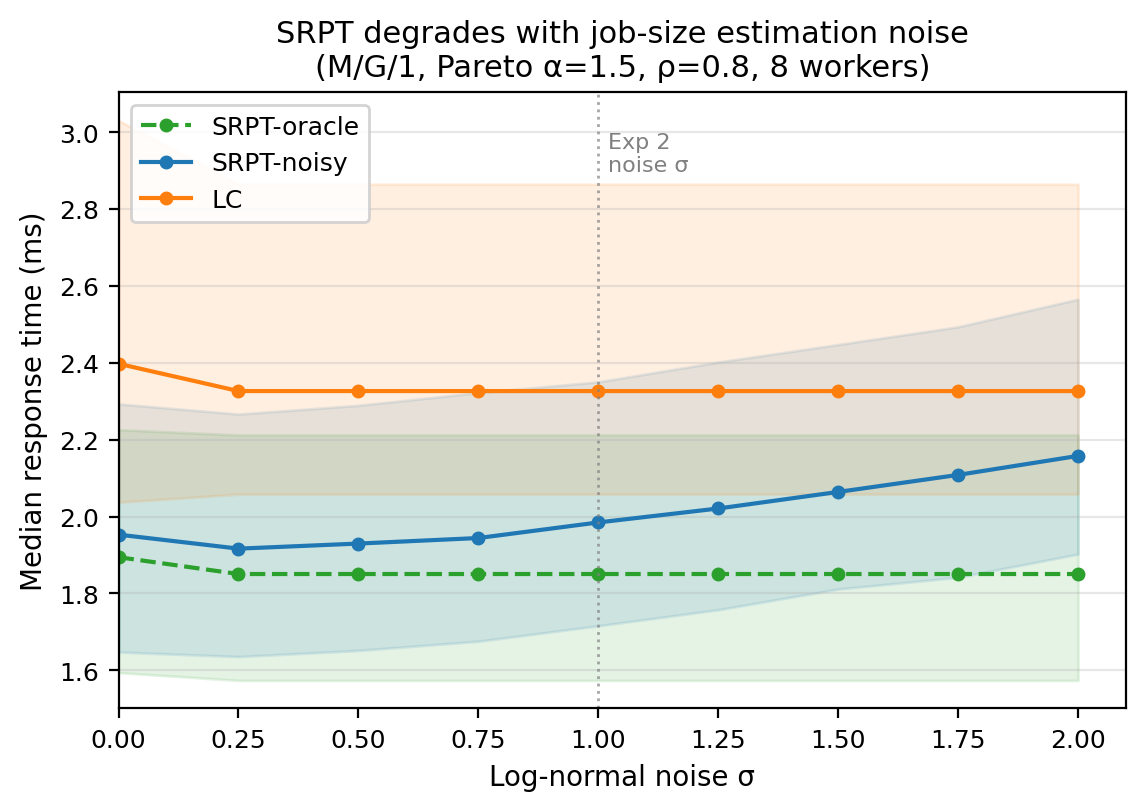
\includegraphics[width=\linewidth]{fig1_noise_sweep}
  \caption{%
    \textbf{SRPT degrades with estimation noise.}
    Median mean response time (50 seeds) versus log-normal noise $\sigma$
    for four baseline strategies.
    SRPT-oracle uses true job sizes and serves as a performance ceiling.
    SRPT-noisy degrades monotonically with $\sigma$.
    Least Connections and Random are unaffected because they do not
    use size estimates.
    The vertical line at $\sigma{=}1.0$ marks the operating point
    used in the LLM evaluation.
  }
  \label{fig:noise-sweep}
\end{figure}

\paragraph{The ideal correction.}
The SRPT failure stems from $\mathrm{ERW}_w$ systematically
underestimating the load on workers with underestimated large jobs.
An alternative, noise-free signal for remaining work is
$c_w \cdot E[S]$, where $c_w = \texttt{connections[w]}$ is the exact
active job count and $E[S]{=}1$\,ms is the known mean service time.
This signal cannot be made arbitrarily small by underestimation because
it depends only on counts, not on size estimates.
A corrected score that blends both signals,
\begin{equation}
  \tilde{s}_w = \mathrm{ERW}_w + \hat{S}_\text{new} + c_w \cdot E[S],
  \label{eq:correction}
\end{equation}
adds a floor term proportional to the number of active jobs.
When $\mathrm{ERW}_w$ is severely underestimated, the floor term
prevents worker $w$ from appearing idle, limiting the accumulation
of phantom-underload traffic.
An equivalent variant enforces a hard floor:
$\tilde{s}_w = \max(\mathrm{ERW}_w,\; c_w \cdot E[S]) + \hat{S}_\text{new}$,
which discards $\mathrm{ERW}_w$ entirely when the connection-count
estimate is larger.

\subsection{Baselines}
\label{sec:exp2-baselines}

We compare four reference policies, each evaluated over 20 seeds:

\begin{itemize}
  \item \textbf{SRPT-oracle.} Route to $\arg\min_w
    \bigl(\mathrm{TRW}_w + S_\text{new}\bigr)$, where
    $\mathrm{TRW}_w$ is the true total remaining work using exact
    job sizes.
    Achieves median 1.79\,ms; serves as a performance ceiling.
  \item \textbf{SRPT-noisy.} Route to $\arg\min_w
    \bigl(\mathrm{ERW}_w + \hat{S}_\text{new}\bigr)$, using
    noisy estimates throughout.
    Achieves median 1.94\,ms.
  \item \textbf{Least Connections (LC).} Route to $\arg\min_w c_w$,
    breaking ties randomly.
    Ignores size estimates entirely; achieves median 2.35\,ms.
  \item \textbf{Random.} Route uniformly at random.
    Achieves median 35.8\,ms; a weak baseline included to confirm
    that LLM-generated functions are not trivially degenerate.
\end{itemize}

\subsection{LLM Evaluation}
\label{sec:exp2-llms}

We use the same six models and the same prompting protocol as
Experiment~1, adapted to the new interface.
The prompt describes the SRPT failure mode explicitly: it explains
that $\mathrm{ERW}_w$ is a frozen accumulated sum, not a running
estimate, and that severely underestimated jobs make a worker appear
nearly idle throughout their service.
We do not suggest a correction strategy.

We generate 100 trials per model.
A trial is valid if the function parses, executes without error,
and does not fall back to a baseline dispatcher on every call
(fallback rate~$< 1.0$).
We exclude fallback-dominated trials because their measured
performance reflects the fallback strategy, not the LLM's intended
logic.
Table~\ref{tab:exp2-results} reports parse rates and valid trial
counts after this filter.

\begin{table}[H]
\centering
\caption{%
  Experiment~2 results (valid trials after filtering fallback-dominated
  runs; models with $n{<}5$ are reported for completeness but are too
  small for reliable inference).
  LLM rows are ordered by valid trial count.
  Baselines are evaluated over 20 independent seeds.
  Lower median mean response time is better.
}
\label{tab:exp2-results}
\smallskip
\begin{tabular}{lrrrr}
\toprule
\textbf{Strategy / Model} & \textbf{Parse\%} & \textbf{$n$ valid} &
  \textbf{Med.\ RT (ms)} & \textbf{IQR (ms)} \\
\midrule
\multicolumn{5}{l}{\textit{Baselines (20 seeds each)}} \\
\quad SRPT-oracle  & --- & --- & 1.79 & [1.55,\;2.10] \\
\quad SRPT-noisy   & --- & --- & 1.94 & [1.66,\;2.26] \\
\quad LC           & --- & --- & 2.35 & [1.91,\;2.66] \\
\quad Random       & --- & --- & 35.8 & [25.0,\;76.4] \\
\midrule
\multicolumn{5}{l}{\textit{LLM-generated dispatchers}} \\
\quad Qwen3-1.7B       &  1\% &  0 & ---  & --- \\
\quad Qwen3-8B         &  6\% &  1 & 1.65 & --- \\
\quad Qwen3-4B         & 26\% &  6 & 2.47 & [1.76,\;3.16] \\
\quad DeepSeek-R1 (8B) & 27\% & 16 & 2.03 & [1.88,\;2.41] \\
\quad gpt-oss-20b      & 36\% & 30 & 2.02 & [1.76,\;3.15] \\
\quad Qwen3-14B        & 50\% & 50 & 2.44 & [1.93,\;3.49] \\
\bottomrule
\end{tabular}
\end{table}

\subsection{Results}
\label{sec:exp2-results}

\paragraph{Scale determines code validity, not performance rank.}
Parse rates and valid trial counts broadly increase with model scale,
though not monotonically:
Qwen3-1.7B produces no valid simulations.
Qwen3-4B (26\% parse rate, 6 valid trials) outperforms the larger
Qwen3-8B (6\%, 1 trial), suggesting that architecture and training
matter alongside raw parameter count.
gpt-oss-20b and DeepSeek-R1 reach 27--36\% parse rates with 16--30
valid trials, and Qwen3-14B achieves the highest parse rate at 50\%
(50 valid trials), giving sufficient sample sizes for inference.

Among models with adequate samples, the ranking does not follow
parameter count.
gpt-oss-20b (median 2.02\,ms) and DeepSeek-R1 (2.03\,ms) achieve
similar performance close to SRPT-noisy (1.94\,ms), while the larger
Qwen3-14B (2.44\,ms) sits closer to LC.
Figure~\ref{fig:exp2-main} shows the full per-model distributions.

\begin{figure}[H]
  \centering
  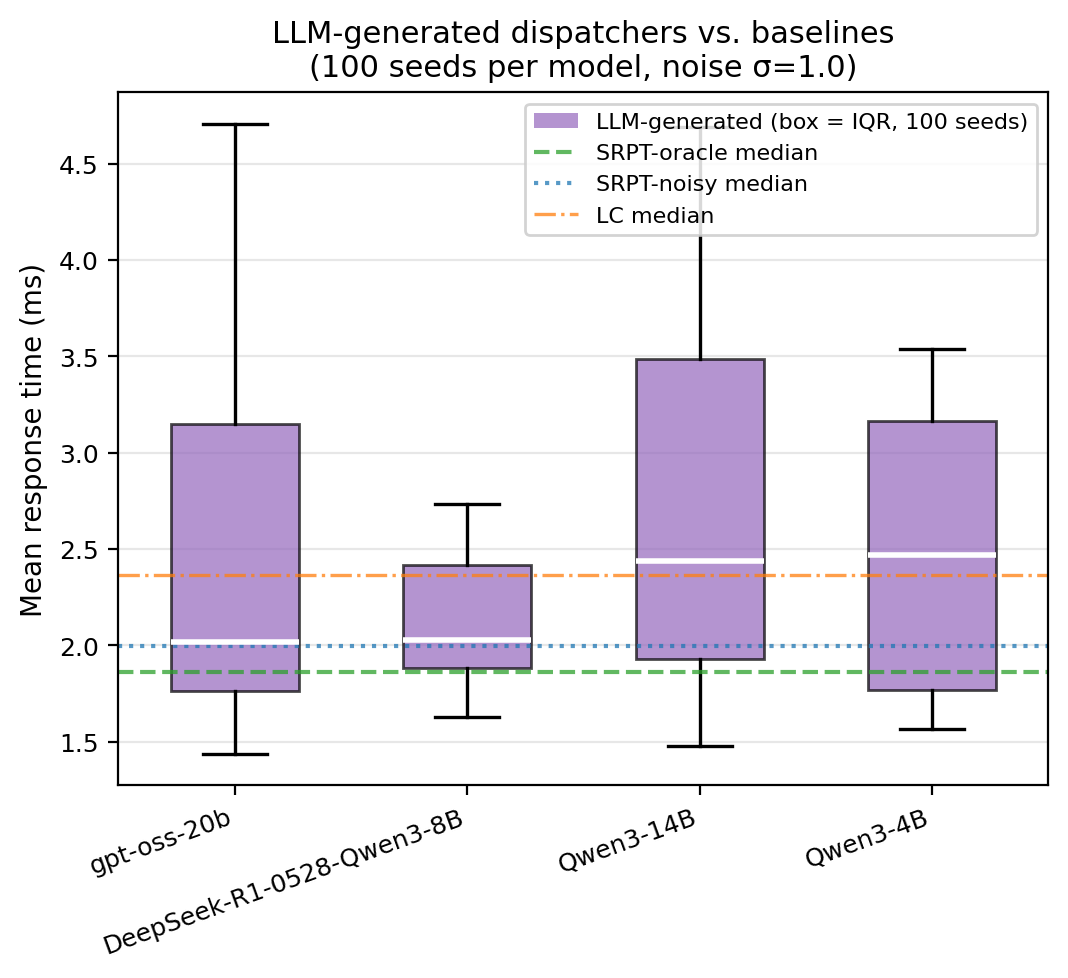
\includegraphics[width=\linewidth]{fig2_main_results}
  \caption{%
    \textbf{Per-model response time distributions in Experiment~2.}
    Box plots show the spread of mean response time across valid
    trials (100 seeds each, fallback-dominated trials excluded).
    Dashed reference lines mark the four baseline medians.
    gpt-oss-20b and DeepSeek-R1 cluster near SRPT-noisy;
    Qwen3-14B shows wider variance.
    Models with $n{<}5$ valid trials are omitted.
  }
  \label{fig:exp2-main}
\end{figure}

\paragraph{Models converge on two distinct strategies.}
Every valid trial falls into one of two strategy classes.
\emph{Both-signals} functions (84 trials, median 2.06\,ms) use a
combination of $\mathrm{ERW}_w$ and $c_w$, corresponding to some
form of the correction in Equation~\eqref{eq:correction}.
\emph{LC-only} functions (19 trials, median 2.58\,ms) route solely
by connection count, effectively reimplementing the LC baseline.
No valid trial implements a pure SRPT-only strategy,
despite the prompt showing SRPT as the starting point.
Models told that SRPT's estimates are unreliable consistently chose
to down-weight or abandon the size-estimate signal; the better
outcome is to correct it rather than discard it, which the
both-signals class does.

\paragraph{The best functions independently discover bias correction.}
Sorting all 103 valid, non-fallback trials by mean response time and
removing exact source-code duplicates yields five unique
top-performing functions, all belonging to the both-signals class.
Two structurally distinct variants appear repeatedly:
\begin{itemize}
  \item \textbf{Additive penalty}
    (ranks 1, 3, 4; primarily from gpt-oss-20b):
    $\tilde{s}_w = \mathrm{ERW}_w + \hat{S}_\text{new}
      + c_w \cdot 1.0$
  \item \textbf{Floor correction}
    (ranks 2, 5; primarily from Qwen3-14B):
    $\tilde{s}_w = \max(\mathrm{ERW}_w,\;
      c_w \cdot 1.0) + \hat{S}_\text{new}$
\end{itemize}
Both use the coefficient 1.0\,ms, equal to $E[S]$, the mean service
time stated in the prompt.
The additive penalty blends both signals; the floor correction
replaces $\mathrm{ERW}_w$ with $c_w \cdot E[S]$ whenever the latter
is larger.
These functions independently reconstruct the correction derived in
Section~\ref{sec:exp2-math} from first principles.

To evaluate robustly, we re-run each of the five unique functions
over 20 fresh seeds (the same 20 seeds used for the baselines in
Table~\ref{tab:exp2-results}).
The top two functions achieve median mean response times of
1.88\,ms and 1.90\,ms respectively, between SRPT-oracle (1.79\,ms)
and SRPT-noisy (1.94\,ms).
Figure~\ref{fig:exp2-best} shows the code alongside the performance
comparison.

\begin{figure}[H]
  \centering
  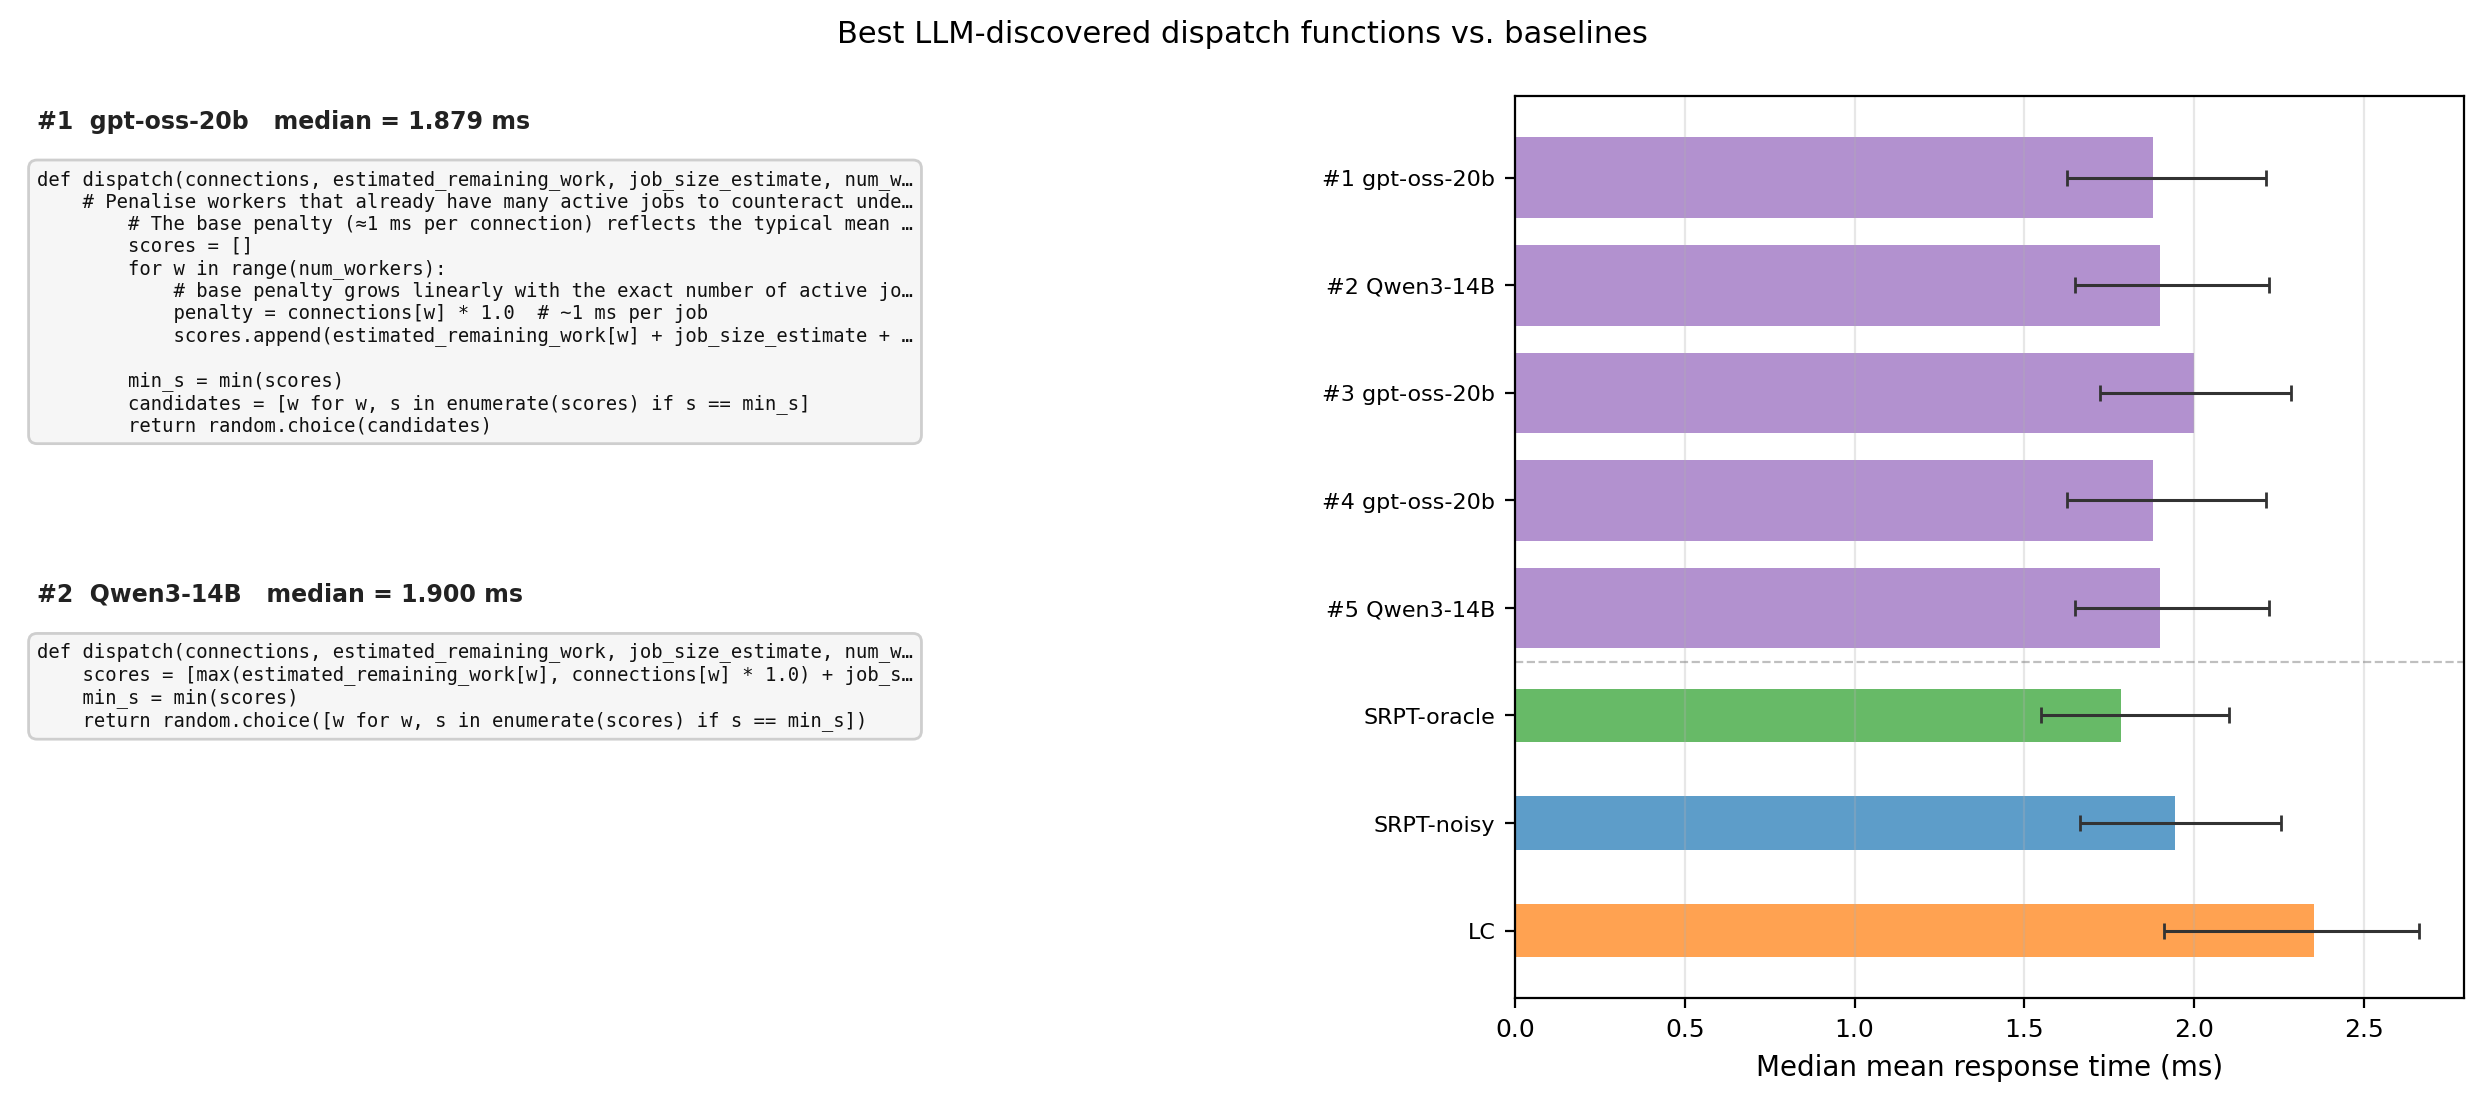
\includegraphics[width=\linewidth]{fig6_best_functions}
  \caption{%
    \textbf{Best LLM-discovered dispatch functions.}
    \emph{Left:} Source code for the two top-performing unique
    functions.
    Both independently discover a connection-count correction to the
    SRPT score; they differ only in whether the correction is additive
    or acts as a floor.
    \emph{Right:} Robust performance comparison (20 seeds each)
    of all five top functions against the four baselines.
    The best two functions fall between SRPT-oracle and SRPT-noisy.
    Error bars show the interquartile range.
  }
  \label{fig:exp2-best}
\end{figure}

These results are best-case: the functions shown are the top entries
from a sorted list of 73 unique valid functions, and they were
discovered inconsistently.
gpt-oss-20b produced 30 valid trials; 3 of them rank in the top 5
while others perform near the LC baseline.
Qwen3-14B produced 50 valid trials with wider variance.
The typical performance of both models is 2.0--2.4\,ms, not 1.88\,ms.
LLMs can synthesize the correct correction when given a description
of the failure mode, but not reliably: the best functions were
discovered in 3 of 30 trials for the top model, not consistently.

% ============================================================
\section{Discussion}
\label{sec:discussion}

\paragraph{Zero-shot generation versus iterative algorithm search.}
Recent work on AI-Driven Research for Systems
(ADRS)~\citep{cheng2025barbarians} demonstrates that LLM-driven
algorithm discovery can match or exceed human-designed baselines
across a range of systems performance problems, including load
balancing, cloud scheduling, and database query optimization.
Related systems such as AlphaEvolve~\citep{novikov2025alphaevolve}
and FunSearch~\citep{fawzi2024funsearch} report similar gains on
combinatorial and algorithmic tasks.
The positive findings of these works may appear to contradict the
largely negative results reported here, but the difference is
methodological rather than a disagreement about LLM capability.

ADRS operates as an iterative search: in each round a solution
generator proposes candidate algorithms, an evaluator scores them
against a simulator, and the resulting scores, along with
qualitative feedback, are fed back into the next generation prompt.
Over hundreds of such iterations, the feedback loop guides the
search toward progressively better solutions, concentrating
probability mass around strategies that the simulator rewards.
Our experiments can be understood as the first rollout of the ADRS
loop: the prompt is issued once, samples are drawn at temperature~1,
and the results are never fed back to refine the prompt.
There is no iteration, no evaluator score returned to the model, and
no continual refinement of the generation context.
The ADRS results establish what is achievable once that feedback loop
runs to convergence; our results establish what a practitioner
receives before it starts.

Experiment~2 makes the relationship particularly clear.
\citet{cheng2025barbarians} identify three components a prompt must
supply for effective algorithm evolution: a precise problem
description, a stated optimisation objective, and context about the
system and its failure modes.
Experiment~2 satisfies all three: it describes the SRPT routing
setting and the noisy-estimate failure mode in detail, states the
objective (reduce mean response time), and provides the reference
SRPT implementation as a starting point.
This prompt structure closely mirrors what ADRS case studies use.
The critical missing ingredient in our setting is the iteration
loop: without an evaluator returning scores to guide subsequent
generations, the model must discover the correct correction in a
single forward pass.
The results are consistent with this framing.
The best functions in Experiment~2 do recover the correction
derived in Section~\ref{sec:exp2-math}, and they use the
coefficient equal to the mean service time stated in the
prompt, indicating that the model reads and applies the failure
description rather than pattern-matching to the interface.
But these functions appear in only 3 of 30 trials for the best-
performing model.
In an ADRS pipeline even this sparse positive signal is sufficient:
a few high-scoring solutions in early rounds provide the feedback
needed to concentrate search toward the correct strategy.
In the zero-shot regime, the same sparsity means a practitioner is
more likely than not to receive a suboptimal function.

A final pattern is relevant to the boundary conditions of iterative
search itself.
Across both experiments, every function that beats the best
classical baseline originates from one of the two largest models
tested, gpt-oss-20b or Qwen3-14B.
The smaller models (Qwen3-1.7B, Qwen3-4B, Qwen3-8B, and
DeepSeek-R1) do not produce a single solution that clears this bar
in either experiment.
This is consistent with a minimum capability requirement for
iterative search to be productive: if a model cannot generate even
one high-quality solution across many independent trials,
an iterative loop that relies on evaluator feedback from those
solutions would receive no informative signal from which to improve.
The parallel to policy optimisation in reinforcement learning is
direct: a policy that assigns near-zero probability to high-reward
actions provides no usable gradient regardless of the number of
training iterations.
Scale may therefore determine not only whether a model produces
valid, executable code (the threshold effect discussed below) but
also whether it is capable of seeding a productive iterative search
at all.
ADRS-style iteration, in other words, amplifies a capability that
already exists in sufficiently large models; it cannot substitute
for it.

That said, the zero-shot regime is arguably the more common one in
practice.
Most engineers who consult an LLM for algorithm advice do so by
asking a question, not by running a simulation-backed optimisation
loop.
Setting up an evaluator, defining a scoring function, and running
hundreds of iterations requires engineering effort that is rarely
available when the goal is simply to get a better dispatch function
quickly.
The median and average-case performance measured in our experiments
therefore reflects what practitioners typically encounter: on
average, the output of a zero-shot query performs worse than the
algorithm it is meant to replace, and human review before deployment
is warranted.

\paragraph{No model reliably beats the best baseline.}
The central finding across both experiments is that LLM-generated
dispatch functions do not reliably improve on the best available
classical baseline.
In Experiment~1, every model's median performance is worse than
Random, meaning the typical LLM output is actively harmed by the
information it uses.
In Experiment~2, median performance sits between LC and SRPT-noisy;
improvements over SRPT-noisy are confined to the top few functions
out of over a hundred trials.
A practitioner who deployed a randomly sampled LLM-generated function
would, in expectation, get worse performance than if they had kept
the original algorithm.

The two experiments differ in \emph{how bad} the typical output is.
In Experiment~2 the task is more forgiving: routing by connection
count alone is reasonable, so abandoning ERW is not catastrophic.
In Experiment~1, using heartbeat age incorrectly is strictly worse
than ignoring it, so more of the strategy space leads to actively
harmful results.
But in both cases, the median LLM output falls short of what a
careful algorithm designer would produce.

\paragraph{Scale as a threshold, not a gradient.}
In both experiments, scale acts as a threshold rather than a
continuous performance gradient.
Models below roughly 8--14B parameters rarely produce valid, non-
fallback dispatchers at all.
Above that threshold, model size does not appear to correlate with
median response time: Qwen3-14B, the largest Qwen3 model tested,
does not outperform gpt-oss-20b in median performance despite having
more parameters, and DeepSeek-R1 matches gpt-oss-20b without clearly
exceeding it.

Where scale does seem to matter is at the extremes.
Smaller models tend to generate more syntactically broken or
semantically incoherent functions, pulling down their worst-case
performance.
Larger models occasionally discover high-quality solutions that
smaller models never reach, even though their typical output is
no better.
This asymmetry suggests that scale increases the ceiling on best-case
solutions without consistently raising the floor.

This pattern raises a natural question about the underlying cause.
The inconsistency between occasional correct solutions and poor
median performance may reflect a generalization failure in the
reinforcement learning stage of these models' training: RLHF or
RLVR reward signals optimized on common code and reasoning tasks may
not transfer reliably to out-of-distribution problems like stochastic
load balancing.
If so, the largest models carry latent knowledge of the correct strategy,
visible in the rare trials that get it right, but cannot sample it
consistently because the policy was not shaped by feedback from
this problem class.

\paragraph{Describing the failure mode helps.}
The two experiments differ in one key respect beyond the failure mode
itself: Experiment~2's prompt explicitly names the phantom-underload
mechanism, while Experiment~1's prompt provides only the interface
and system parameters.
The best-discovered functions in Experiment~2 correct exactly the
described failure, using a coefficient ($1.0$\,ms) equal to the
stated mean service time, indicating that the model is reading and
applying the failure description rather than pattern-matching to the
interface.
This asymmetry explains the gap in discovery rates: Experiment~2
yields more top-performing solutions despite presenting a harder
optimization landscape.
A clean ablation (adding an explicit thundering-herd description to
Experiment~1, or withholding the ERW-freeze explanation from
Experiment~2) would isolate how much of the gap is attributable
to prompt framing versus task difficulty.

\paragraph{Limitations.}
Valid trial counts for small models (Qwen3-4B: $n{=}6$;
Qwen3-8B: $n{=}1$) are too small for reliable inference in
Experiment~2 and should be treated as qualitative.
All results are from a single prompt template; different prompts
may yield different strategy distributions.
The simulation uses a fixed set of parameters ($N{=}8$, $\rho{=}0.8$,
$\alpha{=}1.5$); generalization to other operating points is not tested.

\paragraph{Directions for future work.}
Several open questions follow directly from these results.
First, how robust are LLM-generated dispatch functions to prompt
variation? Small changes in wording, problem framing, or the amount
of context provided may substantially shift the strategy distribution;
a systematic prompt sensitivity study would clarify how much the
current results depend on the specific templates used.
Second, how should synthetic benchmarks for load balancing be
constructed to capture the diversity of real-world scenarios?
The two setups studied here (heartbeat staleness and noisy SRPT) are
representative but not exhaustive; a richer template library spanning
different arrival models, service distributions, and information
structures would enable more general evaluation.
Third, and most directly motivated by the RL generalization
hypothesis above: can reinforcement learning with a simulator as
the reward signal improve LLM load-balancing capabilities?
Using the discrete-event simulation itself as a judge, scoring
generated dispatch functions by the queue standard deviation or mean
response time they achieve, would provide a task-specific reward
signal absent from standard training, and could close the gap between
occasional correct solutions and consistently good ones.

% ============================================================
\section{Conclusion}
\label{sec:conclusion}

We evaluated six LLMs on two load-balancing synthesis tasks designed
to reflect a common practical situation: a practitioner knows a
standard algorithm exists but suspects it is underperforming, and
asks an LLM for a better alternative.

The answer, across both experiments, is that the LLM should not be
trusted blindly.
No model reliably beats the best available baseline in median
performance, and the typical LLM-generated function performs worse
than the baseline it is meant to improve.
Scale determines whether a model can produce valid code at all
(roughly 8B parameters is the threshold) but does not predict
median quality above that threshold.
Larger models do occasionally discover correct solutions, but they
do so inconsistently: the right answer appears in a small minority
of trials, not as the expected output.

Providing an explicit description of the failure mode substantially
increases the rate of correct solutions, suggesting that LLMs have
the underlying capability to fix described problems but not to
diagnose them from scratch.
The most direct next steps are to measure how much of this gap is
driven by prompt framing versus task difficulty, and to explore
whether task-specific reinforcement learning, using the simulator
itself as the reward signal, can close the gap between occasional
correct solutions and consistently reliable ones.

% ============================================================
\newpage
\bibliographystyle{abbrvnat}
\bibliography{references}

% ============================================================
\appendix
\section{Appendix: LLM Prompts}
\label{app:prompts}

Both experiments use the same system prompt and differ only in the user prompt.

\paragraph{System prompt (both experiments).}
\begin{lstlisting}
You are an expert in distributed systems and load balancing.
\end{lstlisting}

\subsection{Experiment 1: Age-Aware Dispatching under Heartbeat Staleness}

\begin{lstlisting}
Write the body of a dispatch function for a distributed system
with {num_workers} workers.

System parameters:
- Poisson job arrivals, total utilisation ~80%
- Exponential service times, mean 1 ms
- Each worker independently sends a heartbeat every ~20 ms;
  heartbeats arrive 1-5 ms later, so each worker's reported
  state has a different age

Function signature:
  def dispatch(queue_lengths: list[int],
               queue_ages_ms: list[float],
               num_workers: int) -> int

  queue_lengths[w]  -- queue depth reported in worker w's
                       last heartbeat
  queue_ages_ms[w]  -- ms elapsed since that heartbeat arrived
  num_workers       -- number of workers

Rules:
- Ages typically range from ~1 ms (just after a heartbeat)
  to ~25 ms (just before the next)
- Return the index of the worker to route the next job to
- Write ONLY the function body (no def line, no imports;
  `random` and `math` are available)
- Wrap the code in <code> and </code> tags
- No text outside the tags
\end{lstlisting}

\subsection{Experiment 2: Noisy SRPT Dispatching with Heavy-Tailed Jobs}

\begin{lstlisting}
You are improving a job dispatcher for a server farm with
{num_workers} workers.

The current dispatcher uses SRPT (Shortest Remaining Processing
Time): it routes each incoming job to the worker with the
smallest estimated total remaining work:

    # baseline -- the function you are replacing
    scores = [estimated_remaining_work[w] + job_size_estimate
              for w in range(num_workers)]
    min_s = min(scores)
    return random.choice(
        [w for w, s in enumerate(scores) if s == min_s])

System parameters:
- Poisson arrivals, total utilisation ~80%, {num_workers} workers
- Job service times follow a Pareto distribution (alpha=1.5,
  mean ~1 ms) -- heavy-tailed, high variance, many large jobs
- Job sizes are estimated with log-normal noise (sigma=1.0):
  estimates can be off by 10x

The failure mode of the current dispatcher:
- When a large job (say, 50 ms) is severely underestimated at
  arrival (say, 0.3 ms), estimated_remaining_work for that
  worker stays near 0 for the entire 50 ms service.
- estimated_remaining_work[w] is a frozen accumulated sum: it
  is increased by the noisy estimate when a job ARRIVES and
  decreased by that same estimate when the job DEPARTS. It does
  NOT decrease as a job runs -- so a wildly underestimated job
  makes the worker look nearly empty throughout its real
  service time.
- Result: more and more jobs get routed to the
  secretly-overloaded worker.

Your task: write an improved dispatch function body that
reduces mean job response time.

Function signature:
    def dispatch(connections: list[int],
                 estimated_remaining_work: list[float],
                 job_size_estimate: float,
                 num_workers: int) -> int

    connections[w]              -- EXACT count of active jobs
                                   at worker w (no noise,
                                   no delay)
    estimated_remaining_work[w] -- noisy accumulated estimate
                                   of remaining work at w (ms)
                                   (mean job size ~1 ms;
                                   estimates are biased and
                                   unreliable)
    job_size_estimate           -- noisy estimate of the
                                   incoming job's size (ms)
    num_workers                 -- number of workers

Rules:
- Return the index (0 to num_workers-1) of the worker to
  receive this job
- Write ONLY the function body (no def line, no imports)
- `random`, `math`, and `numpy` (as `np`) are available
- Wrap your solution code in <code> and </code> tags
\end{lstlisting}

\end{document}
